\documentclass[11pt,a4paper, uplatex]{jsarticle}
%
\usepackage{amsmath,amssymb}
\usepackage{bm}
\usepackage[dvipdfmx]{graphicx}
\usepackage{ascmac}
\usepackage{listings}
\usepackage{underscore}
\lstset{
    frame=single,
    numbers=left,
    tabsize=2
}
%
\setlength{\textwidth}{\fullwidth}
\setlength{\textheight}{40\baselineskip}
\addtolength{\textheight}{\topskip}
\setlength{\voffset}{-0.2in}
\setlength{\topmargin}{0pt}
\setlength{\headheight}{0pt}
\setlength{\headsep}{0pt}
%
\newcommand{\divergence}{\mathrm{div}\,}  %ダイバージェンス
\newcommand{\grad}{\mathrm{grad}\,}  %グラディエント
\newcommand{\rot}{\mathrm{rot}\,}  %ローテーション
%
\title{プログラミング言語実験・C言語 第3回課題レポート}
\author{1510151  栁 裕太}
\date{\today}
\begin{document}
\section{課題5}
%
\subsection{サーバーのみ実行時}

\begin{figure}[h]
  \centering
  \caption{サーバーのみ実行した場合のスクリーンショット}
  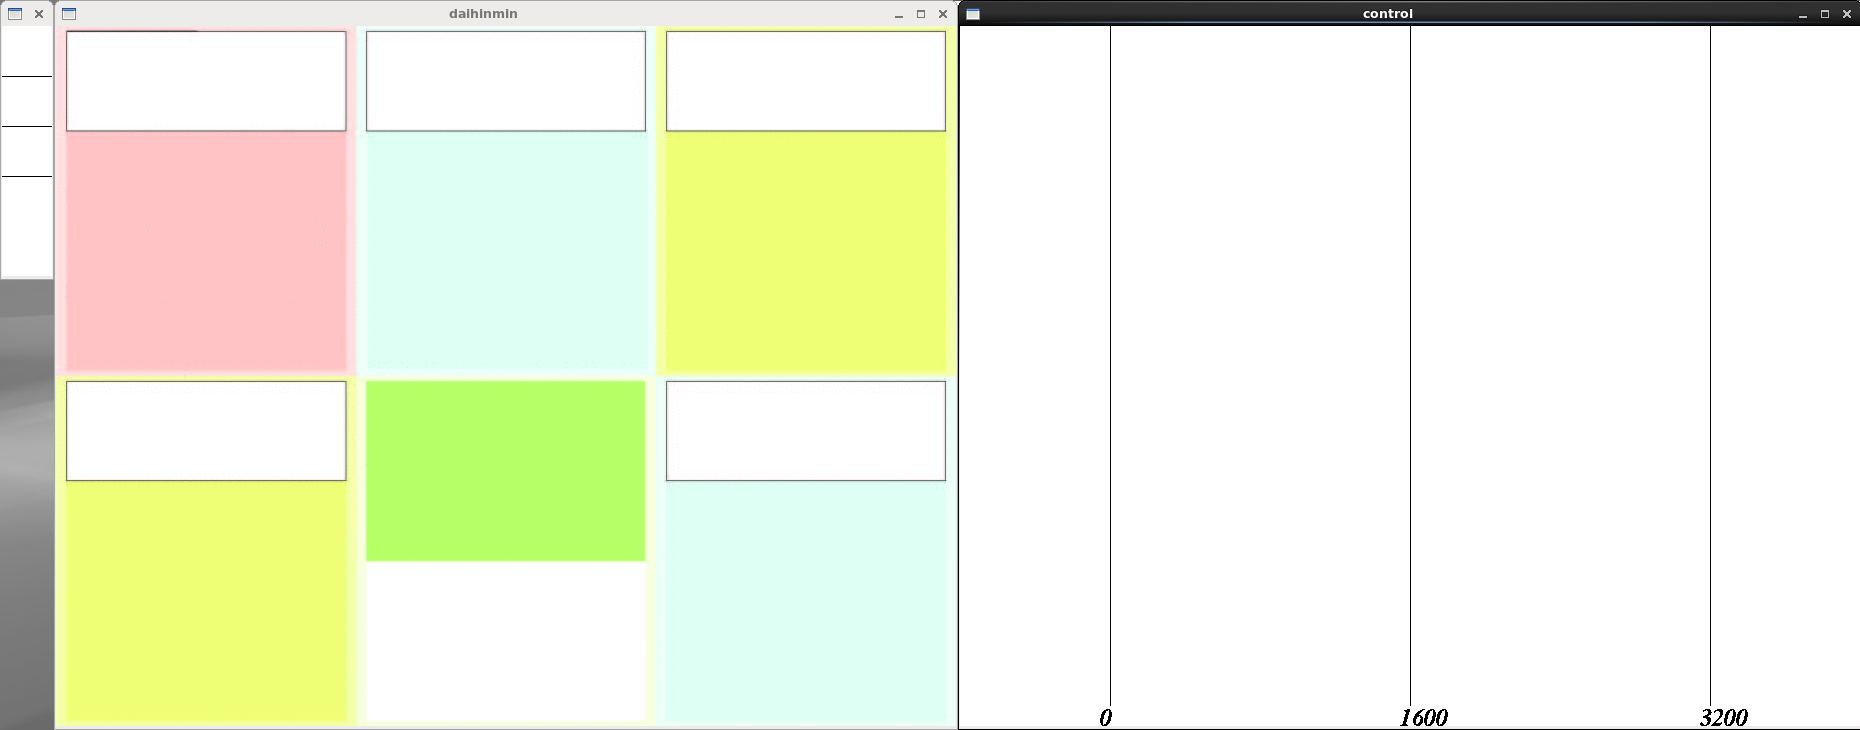
\includegraphics[width=120mm]{ex5-scs.png}
\end{figure}
\subsection{クライアント実行時}

\begin{figure}[h]
  \centering
  \caption{クライアントを5台実行した場合のスクリーンショット}
  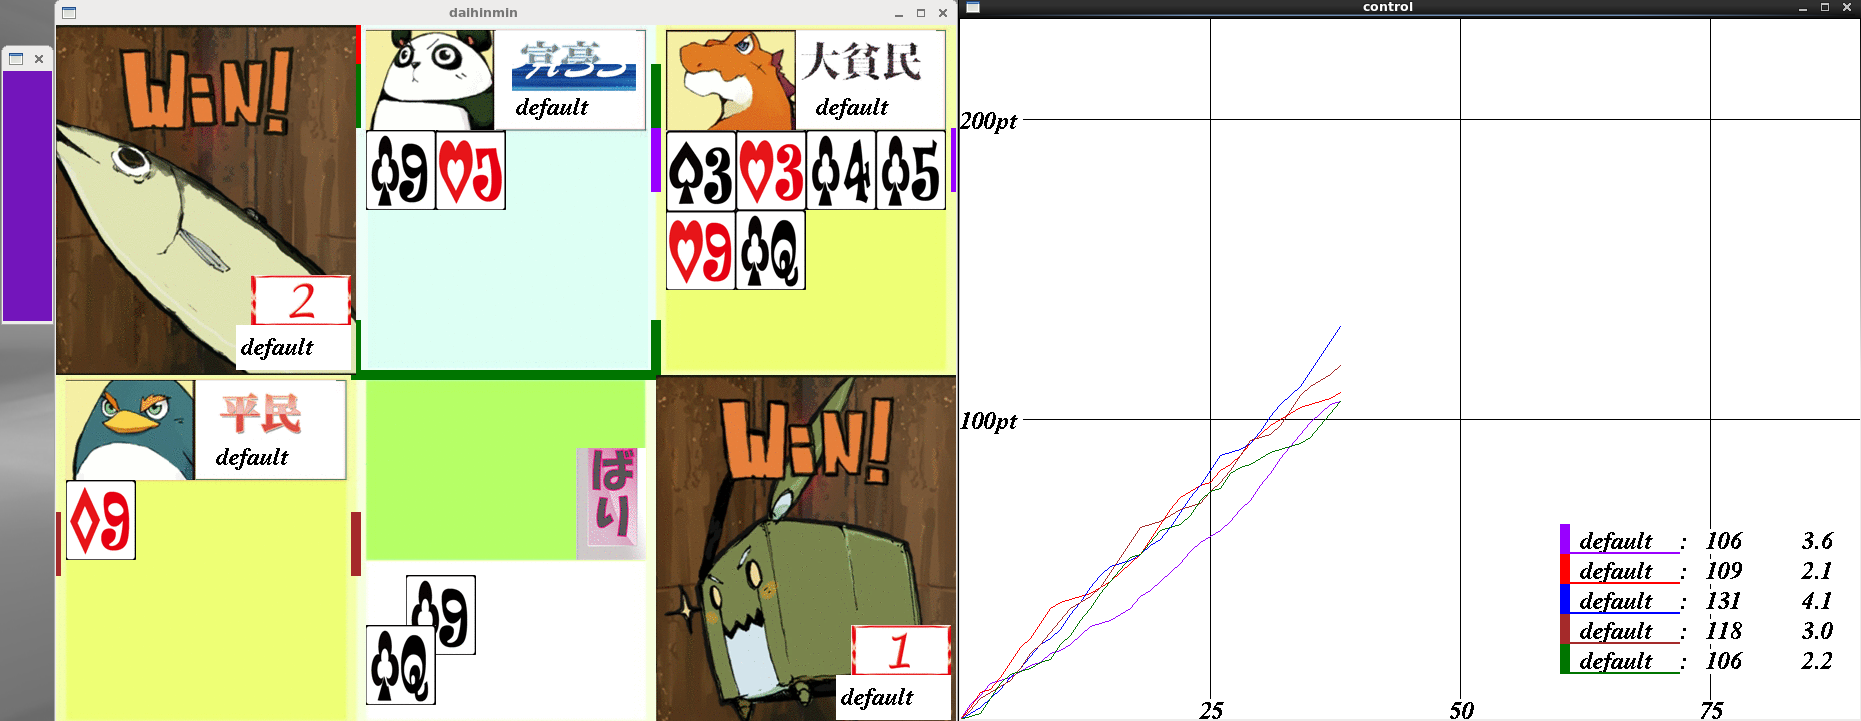
\includegraphics[width=120mm]{./ex5-scs2.png}
\end{figure}

\section{課題6}
%
\subsection{common.c}
%
\subsubsection{copy\_table()}
\paragraph{何の処理?}\mbox{}\\
第二引数の配列の任意の値を第一引数の配列へコピーする処理。
\paragraph{配列への処理内容}\mbox{}\\
第二引数の配列のx行y列の値を第一引数の同じ場所へ代入する
\paragraph{機能実現への決め手}\mbox{}\\
for文を2重にネストし、dst\_cards[i][j]=src\_cards[i][j]とすることで実現が可能となった。
%
\subsubsection{clear\_table()}
\paragraph{何の処理?}\mbox{}\\
引数として受け取ったカードテーブルを初期化する。
\paragraph{配列への処理内容}\mbox{}\\
配列のすべての値を0にする。
\paragraph{機能実現への決め手}\mbox{}\\
for文を2重にネストし、cards[i][j]=0とすることで実現が可能となった。
%
\subsubsection{copy\_cards()}
\paragraph{何の処理?}\mbox{}\\
第二引数の配列のカード情報を第一引数の配列へコピーする処理。
\paragraph{配列への処理内容}\mbox{}\\
第二引数の配列のx行y列(x≦5)の値を第一引数の同じ場所へ代入する
\paragraph{機能実現への決め手}\mbox{}\\
基本的にはcopy\_table()と処理内容は同じである。
1点のみ違いがあり、for文でネストする際にiの制限を8ではなく5とすることで、カード情報のみ指定して初期化することが可能となった。
%
\subsubsection{clear\_cards()}
\paragraph{何の処理?}\mbox{}\\
引数で受け取ったカードテーブルのカード情報の部分のみ初期化する。
\paragraph{配列への処理内容}\mbox{}\\
カードテーブルの第5行までに限り(列は任意)、配列の値を0にする。
\paragraph{機能実現への決め手}\mbox{}\\
基本的にはclear\_table()と処理内容は同じである。
1点のみ違いがあり、for文でネストする際にiの制限を8ではなく5とすることで、カード情報のみ指定して初期化することが可能となった。
%
\subsubsection{diff\_cards()}
\paragraph{何の処理?}\mbox{}\\
ゲーム開始前の貧民・大貧民→大富豪・富豪のカード譲渡において、引数で指定された(search\_low\_card()にて指定された貧民・大貧民持ち札で最も強い1-2枚の)カードを貧民・大貧民の持ち札から削除する処理。
\paragraph{配列への処理内容}\mbox{}\\
第一引数の自分の持ち札を表すcards1と、事前にsearch\_low\_card()にて譲渡=削除すべきカードをcards2[x][y]=1とされた配列を第二引数として受け取った。cards1配列において、cards2[x][y]にて1とされた場所を0にする、つまりcards1[x][y]に0を代入すること。
\paragraph{機能実現への決め手}\mbox{}\\
for文を2重にネストすることで2次元配列cards1[][]全体を探索し、if文として1と指定された場所に限り、cards1の同一の行・列部分に0を代入することで実現可能となった。
%
\subsubsection{or\_cards()}
\paragraph{何の処理?}\mbox{}\\
ゲーム開始前の大富豪・富豪→貧民・大貧民のカード譲渡において、引数で指定された(search\_low\_card()にて指定された貧民・大貧民持ち札で最も強い1-2枚の)カードを富豪・大富豪の持ち札へ追加する処理。
\paragraph{配列への処理内容}\mbox{}\\
第一引数の自分の持ち札を表すcards1と、事前にsearch\_low\_card()にて譲渡=削除すべきカードをcards2[x][y]=1とされた配列を第二引数として受け取った。cards1配列において、cards2[x][y]にて1とされた場所を1にする、つまりcards1[x][y]に1を代入すること。
\paragraph{機能実現への決め手}\mbox{}\\
for文を2重にネストすることで2次元配列cards1[][]全体を探索し、if文として1以上に指定された場所に限り、cards1の同一の行・列部分に1を代入することで実現可能となった。
%
\subsubsection{and\_cards()}
\paragraph{何の処理?}\mbox{}\\
第一引数のcards1配列において、cards2においても1として指定された場所以外をすべて0にする処理。
\paragraph{配列への処理内容}\mbox{}\\
cards1[][]において、cards1とcards2が同じ場所の配列の値がともに1である場合に限り、cards1の該当値を1のままとする。両方共1でないのならば、cards1の該当値は0が代入される。
\paragraph{機能実現への決め手}\mbox{}\\
for文を2重にネストすることで2次元配列cards1[][]全体を探索し、if文としてcards1[i][j]とcards2[i][j]がともに1である場合を\&\&で指定し、その場合はcards[j][i]に1を代入し、それ以外の場合はelseとしてcards[j][i]に0を代入することで、実現可能となった。
%
\subsubsection{not\_cards()}
\paragraph{何の処理?}\mbox{}\\
カードの有無を配列の値を0と1とで入れ替えることで反転する処理。
\paragraph{配列への処理内容}\mbox{}\\
配列の任意の場所の値を0⇄1とで反転している。
\paragraph{機能実現への決め手}\mbox{}\\
for文を2重にネストすることで2次元配列cards[][]全体を探索し、cards[j][i]=1ならば0を、0ならば1をcards[j][i]に代入することで、実現可能となった。
%
\subsubsection{get\_field\_state\_from\_field\_cards()}
\paragraph{何の処理?}\mbox{}\\
場に出ているカードの情報から、現在の場の状況を把握する処理。
\paragraph{配列への処理内容}
\subparagraph{初期段階判定}
cards[i][j]が1である場所を捜し、存在しているカードのスートをfield\_statusのsuit[i]に記録する。すべてのスートを調べた(i=4)ならばjをインクリメントし、iを0に戻す。
\subparagraph{階段判定}
cards[i][j]において、cards[i][J+1]も場に出ている=1である場合、階段が発動していると判定し、field\_statusのis\_sequenceに1を代入する。
\subparagraph{枚数組判定}
階段が不成立の場合(field\_status=0)、まず同一数値における別スートのカードの有無を調べ、存在するならば枚数をカウントするcountをインクリメントし、suit[i]に1を代入する。
存在しなければsuit[i]を代入する。
\subparagraph{革命有無判定}
階段が不成立でjが0または14のとき、革命が発動中ならば、field\_statusのorderに14を代入し、力関係が逆転していることを伝える。
革命中でないのならば、orderには0が代入される。jが0でも14でもない時は、jの値がorderに代入される。
\subparagraph{階段処理判定}
階段が成立中の場合、出されたカードの最大値(j)+1セットの枚数(count)が15を超えず、かつcards[i][j+count]が0でない(場に出ている状態である)間、whileとしてcountをインクリメントする。
その後、革命中ならばfield\_statusのorderにはj+count-1を代入し、革命中でなければjをそのまま代入する。
最後に、field\_statusのsuit[i]に1を代入する。
\subparagraph{場カード有無}
上述のコードによって判定されたcountをfield\_statusのquantityに代入し、更にquantityの数値が0でないのならば、field\_statusのis\_no\_cardに0を代入する。
\paragraph{機能実現への決め手}
\subparagraph{初期段階判定}
whileでjを先に固定し、その後iを0から4までインクリメントしている。スートよりも数字の値の方が重要性が高いため、先に固定することでカード位置の正確な探索が可能になった。
\subparagraph{階段判定}
もし場に同じスートで数字が隣接するカードも出ている場合をif-elseで判別することで可能となった。
\subparagraph{枚数組判定}
jの値は変えずに、iのみ0から4までインクリメントしてcards[i][j]の値を調べることにより、同一数値で何枚カードが存在するか調べることが可能になった。
\subparagraph{革命有無判定}
field\_statusにis\_revという革命有無を記す変数が搭載され、その値の有無によってif-elseを分けることにより、可能なものとなった。
\subparagraph{階段処理判定}
先にスートを固定し、隣接するカードがなくなるまでwhile文を回すことにより、セットで出された階段の枚数の判定が可能になった。
また、革命の有無によって次に出すべき階段のセットの判定を変えることにより、正確に次に出すべきカードを判定することが可能になった。
\subparagraph{場カード有無}
countの値をquantityに移植、さらにquantityが0を超えることをif文でキャッチしその場合is\_no\_cardに0を代入することで新場なのか否かを判別できるようになった。
%
\subsubsection{get\_field\_state\_from\_own\_cards()}
\paragraph{何の処理?}\mbox{}\\
引数として受け取った手札のカードテーブルcards[8][15]から、field\_status所蔵の各状態メンバを操作する処理。
\paragraph{配列への処理内容}
\subparagraph{場カード状況による操作}
場にカードがなければ(cards[5][4]の値の有無)field\_statusのis\_no\_cardに1を、革命状態(cards[5][6]の値の有無)ならばis\_revに1を、縛り状態(cards[5][7]の値の有無)ならis\_lockに1を代入する。
\subparagraph{新場状態の処理}
新たな場となった場合、field\_status内の場に出されたカードセット数quanityや強さを表すorder、縛りを表すis\_lockや出されたカードのスートを表すsuit[]をすべて初期化する。
\subparagraph{プレーヤーステータスの整理}
cards[6][0-4]までが表す手持ちのカード状態をfield\_statusのplayer\_quantity[5]にそれぞれ代入する。
その後、プレーヤーのランク(役職)がcards[6][5-9]までが表しているので、それぞれをplayer\_rank[5]に代入する。
最後に、試合ごとにシャッフルされる座席情報がcards[6][10-14]に記載されているので、それぞれをseat[5]に代入する。
\subparagraph{Joker所持未所持の処理}
cards[4][1]に2が代入されているのはプレーヤーはJokerを所持していることを表しているため、field\_statusのhave\_jokerに1が代入される。
\paragraph{機能実現への決め手}
\subparagraph{場カード状況による操作}
cards[5][4, 6, 7]にそれぞれ場で発生している状態が一括で記載されており、その値を参照することで可能となった。
\subparagraph{新場状態の処理}
操作・参照する変数がfield\_status内メンバで完結しており、わかりやすく処理を書かれることが可能となった。
\subparagraph{プレーヤーステータスの整理}
cards[6][1-14]にプレーヤーのステータスが一括で記載されており、それぞれをfor文で囲むことにより、処理をそれぞれ1行ずつで完結することが可能となった。
\subparagraph{Joker所持未所持の処理}
cards[4][1]にJokerの有無を2を代入することで記載されており、if文で該当値を取得・分岐することで可能となった。
%
\subsubsection{remove\_low\_card()}
\paragraph{何の処理?}\mbox{}\\
配列cards[][]の指定されたエリアの値をすべて0とする処理。
\paragraph{配列への処理内容}\mbox{}\\
第一引数のcards[i][j]において、第二引数で指定されたi以上/以下(jは任意)にて指定された部分を0とする。以上/以下は第三引数rev(革命の有無)が0なら以下、1ならば以上を採用する。
\paragraph{機能実現への決め手}\mbox{}\\
if文で第三引数revの有無で処理を分け、それぞれでfor文を2重にネストして0とするエリアを網羅的に指定することで可能となった。
%
\subsubsection{remove\_suit()}
\paragraph{何の処理?}\mbox{}\\
縛りが発動している際に、指定スート以外のカードを出せないように制限する処理。
\paragraph{配列への処理内容}\mbox{}\\
第一引数cards[i][j]に対して、第二引数suit[i]と第三引数flag(0か1)の合計値が偶数ならば、該当するcards[i][j]のi行中の任意のj列の値を0とする。
\paragraph{機能実現への決め手}\mbox{}\\
for文でまずsuit[i]を調べ、flagとの合計値が偶数であることをif文と剰余演算子でキャッチする。
該当する列を、ネストされたfor文でjを0-14まで動かして0を代入することで可能となった。
%
\subsubsection{count\_cards()}
\paragraph{何の処理?}\mbox{}\\
受け取ったプレーヤーが所持しているカード枚数の合計を返す処理。
\paragraph{配列への処理内容}\mbox{}\\
第一引数として受け取ったcards[i][j]において、i<5, j任意の条件下で0でない=所持しているカードがあれば、枚数をカウントするquantity変数をインクリメントする。
すべてのエリアを参照したら、quantityを返す。
\paragraph{機能実現への決め手}\mbox{}\\
for文を2重にネストし、iの条件を5未満に制限することで純粋にカード所持情報を取得することが可能となった。
%
\subsection{select\_cards.c}
%
\subsubsection{select\_change\_cards()}
\paragraph{何の処理?}\mbox{}\\
試合開始前に行われる貧民・大貧民→大富豪・富豪の最も弱い1-2枚のカードの譲渡を管理する処理。
\paragraph{配列への処理内容}\mbox{}\\
基本的にこの関数は直接配列への代入は行わず、先述のcommon.c記載関数の組み合わせが行われている。
第一引数out\_cards[][]は譲渡するカードを表すため、clear\_table()を呼び出して初期化する。
その後out\_cards[][]と第二引数my\_cards[][]に対して、交換する枚数が指定された第三引数num\_of\_changeの数だけ、search\_low\_card()とdiff\_cards()とor\_cards()を繰り返して、my\_cards[][]からout\_cards[][]に譲渡する。
\paragraph{機能実現への決め手}\mbox{}\\
common.cにて作成した関数を組み合わせ、my\_cards[][]から譲渡するout\_cards[][]を作成することにより、可能なものとなった。
%
\subsubsection{select\_submit\_cards()}
\paragraph{何の処理?}\mbox{}\\
場に出すカードを選択する処理。
\paragraph{配列への処理内容}\mbox{}\\
 まず、場に出すカードを表すカードテーブルselect\_cards[8][15]を定義し、clear\_table()により初期化する。

その後、革命中(field\_status内メンバis\_rev)・新たな場(field\_status内メンバis\_no\_card)によって場に出すカードを指定する関数を使い分けている。使用する関数は以下に表される。

なお、渡す引数はselect_cards, my_cards, field_statusと共通している。
\begin{table}[hbtp]
  \caption{使用する関数名}
  \centering
  \begin{tabular}{lcrr}
    状態 & 通常: is\_rev=0 & 革命: is\_rev=1\\
    新場: is\_no\_card=1  & select_cards\_free & select\_cards\_free\_rev \\
    既存場: is\_no\_card=0  & select\_cards\_restrict & select\_cards\_restrict\_rev \\
  \end{tabular}
\end{table}
\paragraph{機能実現への決め手}\mbox{}\\
上記のように、field\_status内メンバによって呼び出す関数を使い分けることにより、革命・や場の状況に応じて最適なカードを出すことが可能となった。
%
\subsubsection{select\_cards\_free()}
\paragraph{何の処理?}\mbox{}\\
場にカードがなにもないときに呼び出され、手札で最も弱いカードを場に出す処理。
\paragraph{配列への処理内容}\mbox{}\\
daihinmin.cにて定義されたsearch\_low\_card()関数へ提出するカードを記した第一引数select\_cards[][]と、手札を記した第二引数my\_cards[][]と、Jokerを使わないことを表す0をそれぞれ引数として渡している。
\paragraph{機能実現への決め手}\mbox{}\\
daihinmin.cのsearch\_low\_cardへそのまま引数として受け取った配列を渡すことにより、実現可能となった。
%
\subsubsection{select\_cards\_restrict()}
\paragraph{何の処理?}\mbox{}\\
場にカードが既にあるときに呼び出され、更に場の状況に応じて出すことが可能なカードを場に出す処理。
\paragraph{配列への処理内容}\mbox{}\\
 まず、場に出すことができるカードを記載するカードテーブルtmp\_cards[][]配列を定義し、copy\_table関数にて第二引数の手札のカードテーブルmy\_cards[][]配列の内容をコピーする。

その次にif文として第三引数field\_status内メンバis\_sequenceが1のときと、quantityが1のときをそれぞれ検知し、更に縛りの有無によって分岐が用意されているが、中身は実装されていない。

処理が実装されているのは場が単騎のみの場合で、この時に場が縛られている(field\_status内メンバis\_lockの値の有無)かをif文で検知し分岐している。
縛られているときはremove\_suit関数を先に入れてtmp\_cards[][]を縛られたスートに制限する。
その後は両者共通でremove\_low\_card()によって、tmp\_cards[][]内で場のカードより弱いカードを削除する。
最後に、search\_low\_card()にて、場に出せられるカードが記載されたtmp\_cards[][]から最も弱いカードを指定し、第一引数select\_cards[][]に反映する。
\paragraph{機能実現への決め手}\mbox{}\\
まず場の状況が階段・ペア・単騎によって分け、更に縛られている・いない場合によって分けることで、それぞれの状況に応じた処理を実装することが可能となった。
%
\end{document}
